\documentclass[conference]{IEEEtran}
\IEEEoverridecommandlockouts
% The preceding line is only needed to identify funding in the first footnote. If that is unneeded, please comment it out.
\usepackage{cite}
\usepackage{amsmath,amssymb,amsfonts}
\usepackage{algorithmic,algorithm}
\usepackage{graphicx}
\graphicspath{ {./images/} }
\usepackage{textcomp}
\usepackage{xcolor}
\usepackage{lettrine}

\def\BibTeX{{\rm B\kern-.05em{\sc i\kern-.025em b}\kern-.08em
    T\kern-.1667em\lower.7ex\hbox{E}\kern-.125emX}}
\begin{document}

\title{SpotifyClassifier: Music Genre Classification with Big Data\\
}

\author{\IEEEauthorblockN{1\textsuperscript{st} Alex Thornton}
\IEEEauthorblockA{\textit{Dept. of Electrical Engineering} \\
\textit{Columbia University}\\
New York, USA \\
apt2141@columbia.edu}
\and
\IEEEauthorblockN{2\textsuperscript{nd} Elmira Aliyeva}
\IEEEauthorblockA{\textit{Dept. of Computer Science} \\
\textit{Columbia University}\\
New York, USA \\
ae2970@columbia.edu}
\and
\IEEEauthorblockN{3\textsuperscript{rd} Tanvi Pande}
\IEEEauthorblockA{\textit{Dept. of Electrical Engineering} \\
\textit{Columbia University}\\
New York, USA \\
tp2673@columbia.edu}
}

\maketitle
\thispagestyle{plain}
\pagestyle{plain}
\begin{abstract}
Music genre classification is a complex task, which can even be difficult for humans. Using a Spotify Developer account to interface with their API, we have created our own dataset and a music genre classifier capable of identifying song genres across a much larger range of genres and subgenres than previously achieved in academic research. Additionally, we leverage Spotify's pre-processed track metadata, allowing for genre classification with only a song name as an input, rather than an audio mp3 file.
\end{abstract}

\begin{IEEEkeywords}
Music, Classification, Hierarchal Learning, Machine Learning, Big Data Analytics, Supervised Learning
\end{IEEEkeywords}

\section{Introduction}
\lettrine{E}{ach} December 1\textsuperscript{st}, social media explodes with a "Spotify Wrapped" summary of users' preferences over the past year. Individual users can post to Instagram or Tik Tok about their top artists, tracks, genres, as well as more abstract concepts like music aura. Currently, Spotify's API can only provide genre labels for artists, not specific tracks. Our team has combined the power of the Spotify Developer API with big data tools such as Google Cloud Computing, Apache Spark, and machine learning techniques to solve this problem. 

Considering the widespread interest and proliferation of "Spotify Wrapped" posts in 2021, there is a clear business value for being able to predict the genre tastes of individual users, particularly their favorite songs. However, Spotify providing genre labels for only artists does not provide enough granularity. Consider the example of a listener of Taylor Swift enjoying \emph{Trouble (Taylor's Version)} on her 2021 re-release of her popular album \emph{Red (Taylor's Version)}. What genre would this song be classified as? Spotify might be able to point you to an array of genres that Taylor Swift has performed over her career, but this is a very broad list! Entire albums across her discography vary greatly tonally, lyrically, and musically. Figure \ref{fig:TSwiftie} illustrates the vast difference between \emph{Red (Taylor's Version) (2021)} and \emph{Reputation (2017)}.

\begin{figure}[htbp]
\centerline{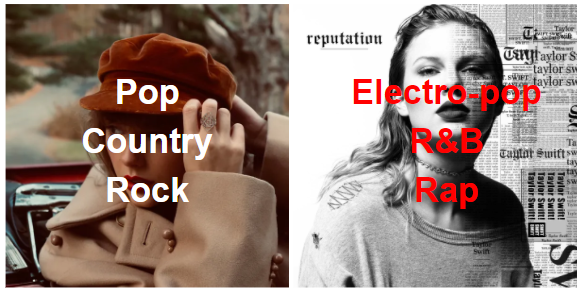
\includegraphics[width=9cm]{images/TSwiftie.png}}
\caption{Red (Taylor's Version) vs. Reputation}
\label{fig:TSwiftie}
\end{figure}

We suspect that on their application backend, Spotify has genre classifications for individual tracks. However, they are likely not providing all their information publicly, and are treating some subset of their data as trade secret. This suspicion is further supported by "Spotify Wrapped" including genres that are not supported for their Developer API. Spofity only supports 126 genres with their Developer API, but have been known to classify music into over 1,300 micro-genres like "grave-wave" and "metropolis" \cite{b1}. To uncover some of the magic of Spotify's classification algorithms, we built our own dataset of labelled tracks using their 'recommendation' feature, and used machine learning to reverse engineer a classification algorithm of our own. 

\section{Related Work}

Starting in 2002,  G. Tzanetakis and P. Cook attempted to use k-nearest neighbors models to perform genre classification on 3 broad genre sets, with an accuracy of around 61\% \cite{b2}. A more recent academic project out of Stanford's CS229 Machine Learning class was able to increase this amount to 80\% for 10 genres, using a CNN trained on the Short Time Fourier Transform (STFT) of song mp3 files from the publicly available GTZAN dataset of 1000 songs \cite{b3}. These examples are able to achieve decent accuracy, as human performance on classification across this range of high level genres is usually around 70\% \cite{b4}.

A more interesting application also comes out of Stanford's CS229 Machine Learning class was able to classify across 4 distinct genres (Christian, Country, Jazz, Metal) by processing the album art, lyrics, and a small audio sample of songs, which they procured using the Spotify Developer API. Processed features were then fed through a recurrent neural network (RNN), Naive Bayes, and other models to achieve over 90\% accuracy. While this is excellent accuracy, the genre selection they used isn't very useful or broad.

Suppose that a user wants to classify the genre of a specific track, but doesn't have access to an mp3 file. The previous examples would be useful if a large enough dataset of mp3 files was labelled, and the user would always have a copy of the music they want to classify. However, the very existence of Spotify as a streaming service indicates a growing movement to separate users from the actual data itself, as opposed to audio marketplace and storage solutions of the early 2000's like iTunes. A much more likely scenario would be a use case where a user knows the name of a track they want to classify, but don't actually own or possess a copy of the music. A clunky implementation for this use case might scrape YouTube and illegally convert the audio to a mp3, then run the raw data through one of the previously mentioned genre classification models. While this might suffice for a proof of concept, we prefer to do things by the book.

Our method embraces big data and the plethora of publicly available metadata through the Spotify Developer API, and can fetch metadata and classify based on the name of a track alone. While genre classification itself isn't a novel application of machine learning, this use case is. Using the Spotify API, our team built our own dataset that leverages over 30,000 individual songs, from 73 distinct genres, and ambitiously has set out to classify genres using this broader, big data approach.

\section{Data}
\subsection{Data Collection}
One of the unique aspects of Spotify's Developer API is its 'recommendation' feature, which can be used to find music that matches a number of criteria, including genres. As of December 2021, Spotify supports a total of 126 genres for recommendation. While Spotify doesn't provide the genre labels for individual tracks, they are able to recommend up to 100 specific tracks for a given seed genre. By requesting recommendations for each supported genre in a loop, and saving off non-repeat tracks until a sufficient number were collected, we were able to construct a labelled dataset of tracks, their Spotify ID, and a corresponding genre label. 

\begin{figure}[htbp]
\centerline{\includegraphics[width=9cm]{images/pitch.png}}
\caption{Audio filter for pitch vectorization}
\label{fig:pitch}
\end{figure}

After tracks were collected and organized with genre labels, we went back to Spotify to collect metadata to serve as features for our model. Available audio features include scores for abstract concepts like 'danceability' to more concrete, quantitative values like tempo and loudness. Features were saved to a json file for each track, and stored in a Google Cloud Storage project. 

\begin{figure}[htbp]
\centerline{\includegraphics[width=9cm]{images/timbre.png}}
\caption{Timbre basis function}
\label{fig:timbre}
\end{figure}

In addition to pre-processed audio features, we also leveraged Spotify's 'Audio-Analysis' and 'Track-Info' calls. Track info is straightforward, allowing us to collect the year of release and relative popularity of tracks, which actually serve as excellent discriminators. A lot more people are listening to Ed Sheeran in 2021 than Mozart, and classic rock music is much more likely to correlate to music written in the 1980s. Audio analysis calls provide in depth analysis of tracks, with 1x12 vectors for each musically distinct 'segment' of a song for pitch and timbre. As songs can have vastly different numbers of unique segments depending on song length, we averaged pitch and timbre to get consistent 1x12 vectors as features. Figures \ref{fig:pitch} and \ref{fig:timbre} show a visual representation of these vectors.

\subsection{Genre Hierarchy}

With a class of genres so large, we clustered 73 of the 126 genres as subgenres under larger 'super-genres'. For example, grunge, emo, and indie could all be subgenres of the 'alternative' super-genre. Initially, we expected to classify based on both super-genre and subgenre, with performance on the former being much better. However, as discussed in the Analysis section, subgenre classification was much more difficult than anticipated. 

\begin{figure}[htbp]
\centerline{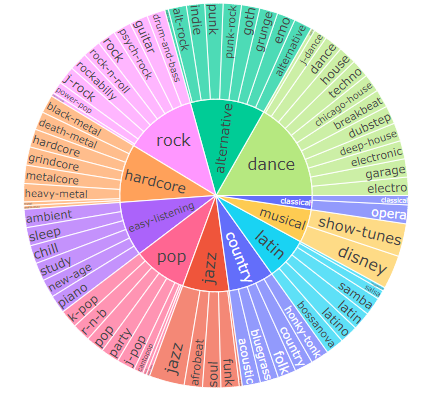
\includegraphics[width=8cm]{images/GenreHierarchy.PNG}}
\caption{Super-genre hierarchy of subgenres}
\label{fig:GenreHierarchy}
\end{figure}

\begin{figure*}
  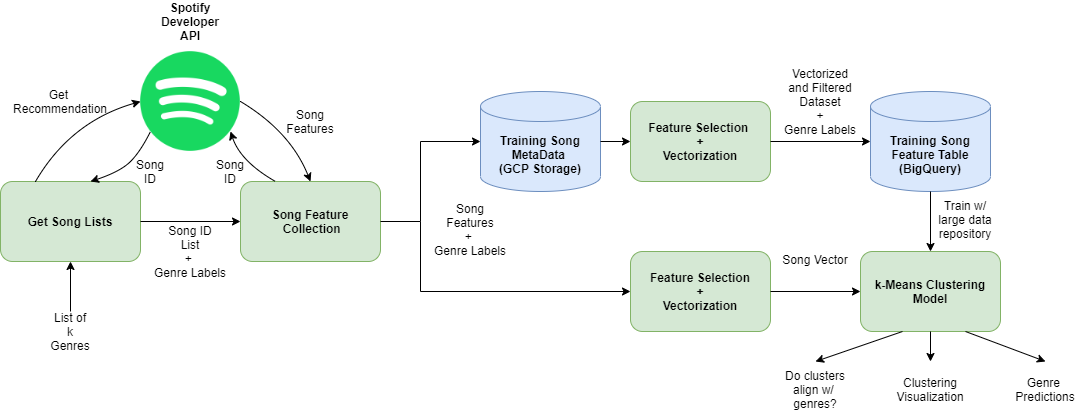
\includegraphics[width=\textwidth]{images/SystemArchitecture.png}
  \caption{System architecture}
  \label{fig:architecture}
\end{figure*}

Approximately 500 songs were collected for each subgenre, creating as balanced a dataset as possible. We realized through trial and error that while many subgenres were able to produce almost 1000 unique tracks after a few hundred API calls (and throwing away repeats each time), some subgenres only had the same 100 tracks for every API call. We ended up tossing out subgenre seeds with only 100 tracks to offer, whittling the 126 supported genres to 73 that had enough tracks and could be categorized nicely into super-genres. We also found that 500 tracks was a good target for track count per subgenre.

An important distinction is that some subgenres could fall under multiple super-genres, like punk-rock being split across alternative and rock. For simplification, we mapped each subgenre to only one super-genre. This simplification would prove problematic later, but served as a solid first pass. The super-genre hierarchy used is shown in Figure \ref{fig:GenreHierarchy}, displayed as a sunburst diagram with subgenres branching radially from their respective super-genre. Additionally, the scale of the diagram is accurate for relative track count between genres within our dataset. The number of samples per subgenre, and number of subgenres per super-genre were carefully selected to create as balanced a dataset as possible.

\section{System Overview}
The system architecture is defined in Figure \ref{fig:architecture}, with scripts in green, cloud storage in blue, and front end in purple. Data collection, as described in previous sections, interacts directly with the Spotify Developer API. Track lists are compiled from recommendations for supported seed genres, and features are collected for each of those tracks. From here, we leveraged Colab / Jupyter notebooks, Google Cloud nodes, and Apache Spark to vectorize and store the features as json files for each song, in directories by subgenre. 

Data from cloud storage was converted to tables in BigQuery, so that we could easily prep and load training, and validation data. We went with an 80:20 split across every subgenre for training / validation. A number of machine learning models were tested against our training data to find the best model for our application, and the \emph{Methods} section describes the results for individual models. This trained model is saved and stored on our Github repository for easy loading into the application.

\begin{figure}[htbp]
\centerline{\includegraphics[width=8cm]{images/Application.png}}
\caption{Mock-up of front end application}
\label{fig:application}
\end{figure}

A stretch goal for our team was to have the end user only interact with the simple purple block, with a clean design and intuitive design. The user enters the track they want to classify into a search bar, and on the back end, we determine the closest match for that track with the Spotify 'Search' call. The features are collected and vectorized similarly as with the training data, and passed through the pre-trained machine learning model for classification. We ended up running out of time for the live demo getting the front end connected to the back end, but do have a mock-up of what an application might look like, as shown in Figure \ref{fig:application}.

\section{Methods}


\section{Analysis}

\begin{algorithm} 
\begin{algorithmic}[H]
\caption{Interconnectedness-Rank}
\STATE I $\gets$ dictionary of zero for all subgenres
\STATE T $\gets$ empty list
\FOR{all $s \in S$}
\FOR{all track-id in s}
\STATE T.append (track-id, subgenre) 
\ENDFOR
\ENDFOR
\STATE T $\gets$ (elements of T w/ $>$ 1 appearance of track-id)
\STATE subgenre-clusters $\gets$ empty hash table
\FOR{ all $t \in T$}
\STATE subgenre-clusters[t[track-id]].append(t[subgenre])
\ENDFOR
\STATE E $\gets$ array of \emph{False} for all subgenres, dimension S x S
\FOR{cluster in subgenre-clusters}
\FOR{all s in cluster}
\STATE I[s] += 1
\ENDFOR
\FOR{all pairs i,j of subgenres in cluster}
\IF {E[i,j] == \emph{False}} 
\STATE E[i,j] = \emph{True}
\ENDIF
\ENDFOR
\ENDFOR
\STATE I[s] = reverse-sort-by-value(I[s])
\RETURN (E, I)
\end{algorithmic}
\end{algorithm}

\subsection{Conclusion}

\begin{figure}[htbp]
\centerline{\includegraphics[width=9cm]{images/SupergenreGraphSquare.PNG}}
\caption{Subgenre overlap visualization}
\label{fig}
\end{figure}




\begin{thebibliography}{00}
\bibitem{b1} N. Patch, Meet the man classifying every genre of music on Spotify, thestar.com. 2016.
\bibitem{b2} G. Tzanetakis and P. Cook. Musical genre classification of audio signals. IEEE Transactions on Speech and Audio Processing, 10(5):293–302, July 2002.
\bibitem{b3} D. Huang, A. Serafini, E. Pugh, \emph{Music Genre Classification}, 2018, Accessed on December 21, 2021. [Online]. Available: \url{http://cs229.stanford.edu/proj2018/report/21.pdf}
\bibitem{b4} Mingwen Dong. Convolutional neural network achieves human-level accuracy in music genre classification. CoRR, abs/1802.09697, 2018.
\bibitem{b5} T. Dammann, K. Haugh, \emph{Genre Classification of Spotify Songs using Lyrics, Audio Previews, and Album Artwork}, 2017, Stanford University

\end{thebibliography}

\end{document}

